\documentclass[tikz,border=4pt]{standalone}
\usepackage[T1]{fontenc}
\usepackage{lmodern}
\usetikzlibrary{circuits.logic.US,calc}
\begin{document}
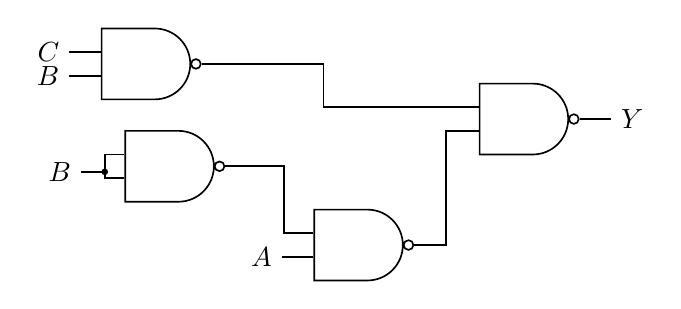
\begin{tikzpicture}[circuit logic US,
  every circuit symbol/.style={draw,minimum width=10mm,minimum height=9mm},
  every node/.style={font=\normalsize},line width=.6pt]
  \node[nand gate US,draw,minimum width=10mm,minimum height=9mm,logic gate inputs=nn] (I1) at (0,1.5) {};
  \node[nand gate US,draw,minimum width=10mm,minimum height=9mm,logic gate inputs=nn] (I2) at (.3,.2) {};
  \node[nand gate US,draw,minimum width=10mm,minimum height=9mm,logic gate inputs=nn] (I3) at (2.7,-.8) {};
  \node[nand gate US,draw,minimum width=10mm,minimum height=9mm,logic gate inputs=nn] (Y) at (4.8,.8) {};
  \draw (I1.input 1) -- ++(-.4,0) node[left] {$C$};
  \draw (I1.input 2) -- ++(-.4,0) node[left] {$B$};
  \coordinate (tap) at ($(I2.input 1)+(-.25,-.22)$);
  \draw (I2.input 1) -- (I2.input 1 -| tap) -- (I2.input 2 -| tap) -- (I2.input 2);
  \draw (tap) -- ++(-.3,0) node[left] {$B$};
  \fill (tap) circle (1.2pt);
  \draw (I1.output) -- ++(1.55,0) |- (Y.input 1);
  \draw (I2.output) -- ++(.75,0) |- (I3.input 1);
  \draw (I3.input 2) -- ++(-.4,0) node[left] {$A$};
  \draw (I3.output) -- ++(.4,0) |- (Y.input 2);
  \draw (Y.output) -- ++(.4,0) node[right] {$Y$};
\end{tikzpicture}
\end{document}
